% -*- latex -*-
%%%%%%%%%%%%%%%%%%%%%%%%%%%%%%%%%%%%%%%%%%%%%%%%%%%%%%%%%%%%%%%%
%%%%
%%%% This TeX file is part of the course
%%%% Introduction to Scientific Programming in C++/Fortran2003
%%%% copyright 2017/8 Victor Eijkhout eijkhout@tacc.utexas.edu
%%%%
%%%% pointer.tex : about pointers
%%%%
%%%%%%%%%%%%%%%%%%%%%%%%%%%%%%%%%%%%%%%%%%%%%%%%%%%%%%%%%%%%%%%%

\Level 0 {What is a pointer}

The term pointer is used to denote a reference to a quantity. The
reason that people like to use C++ and C as high performance languages is
that pointers are actually memory addresses. So you're programming
`close to the bare metal' and are in fargoing control over what your program
does.

\Level 0 {Pointers and addresses, C style}
\label{sec:cderef}

You have learned about variables, and maybe you have a mental concept
of variables as `named memory locations'. That is not too far of:
while you are in the (dynamic) scope of a variable, it corresponds to
a fixed memory location.

\begin{exercise}
  \label{ex:varmemscope}
  When does a variable not always correspond to the same location in
  memory?
\end{exercise}

There is a mechanism of finding the actual address of a variable: you
prefix its name by an ampersand. 
This address is integer-valued, but
its range is actually greater than of the \n{int} type.

\begin{block}{Memory addresses}
  \label{sl:ampersand}
  If you have an
\begin{verbatim}
int i;
\end{verbatim}
then \n{&i} is the address of~\n{i}.

An address is a (long) integer, denoting a memory address. Usually it
is rendered in \indexterm{hexadecimal} notation. C~style:
%
\snippetwithoutput{printfpoint}{pointer}{printfpoint}
%
and C++:
%
\snippetwithoutput{coutpoint}{pointer}{coutpoint}
%\verbatimsnippet{coutpoint}
\end{block}

You could just print out the address of a variable, which is sometimes
useful for debugging. If you want to store the address, you need to
create a variable of the appropriate type. This is done by taking a
type and affixing a star to it.

\begin{block}{Address types}
  \label{sl:intstar}
  The type of `\n{&i}' is \n{int*}, pronounced `int-star',\\
  or more
  formally: `pointer-to-int'.

  You can create variables of this type:
\begin{verbatim}
int i;
int* addr = &i;
\end{verbatim}
\end{block}

Now if you have have a pointer that refers to an int:
\begin{verbatim}
int i;
int *iaddr = &i;
\end{verbatim}
you can use (for instance print) that pointer, which gives you the
address of the variable. If you want the value of the variable that
the pointer points to, you need to \indexterm{dereference} it.

\begin{block}{Dereferencing}
  \label{sl:starderef}
    Using \n{*addr} `dereferences' the pointer: gives the thing it
    points to;\\
    the value of what
    is in the memory location.

\begin{verbatim}
int i;
int* addr = &i;
i = 5;
cout << *addr;
i = 6;
cout << *addr;
\end{verbatim}
This will print~\n{5} and~\n{6}:
\end{block}

\begin{block}{illustration}
  \label{sl:copy-pic}
  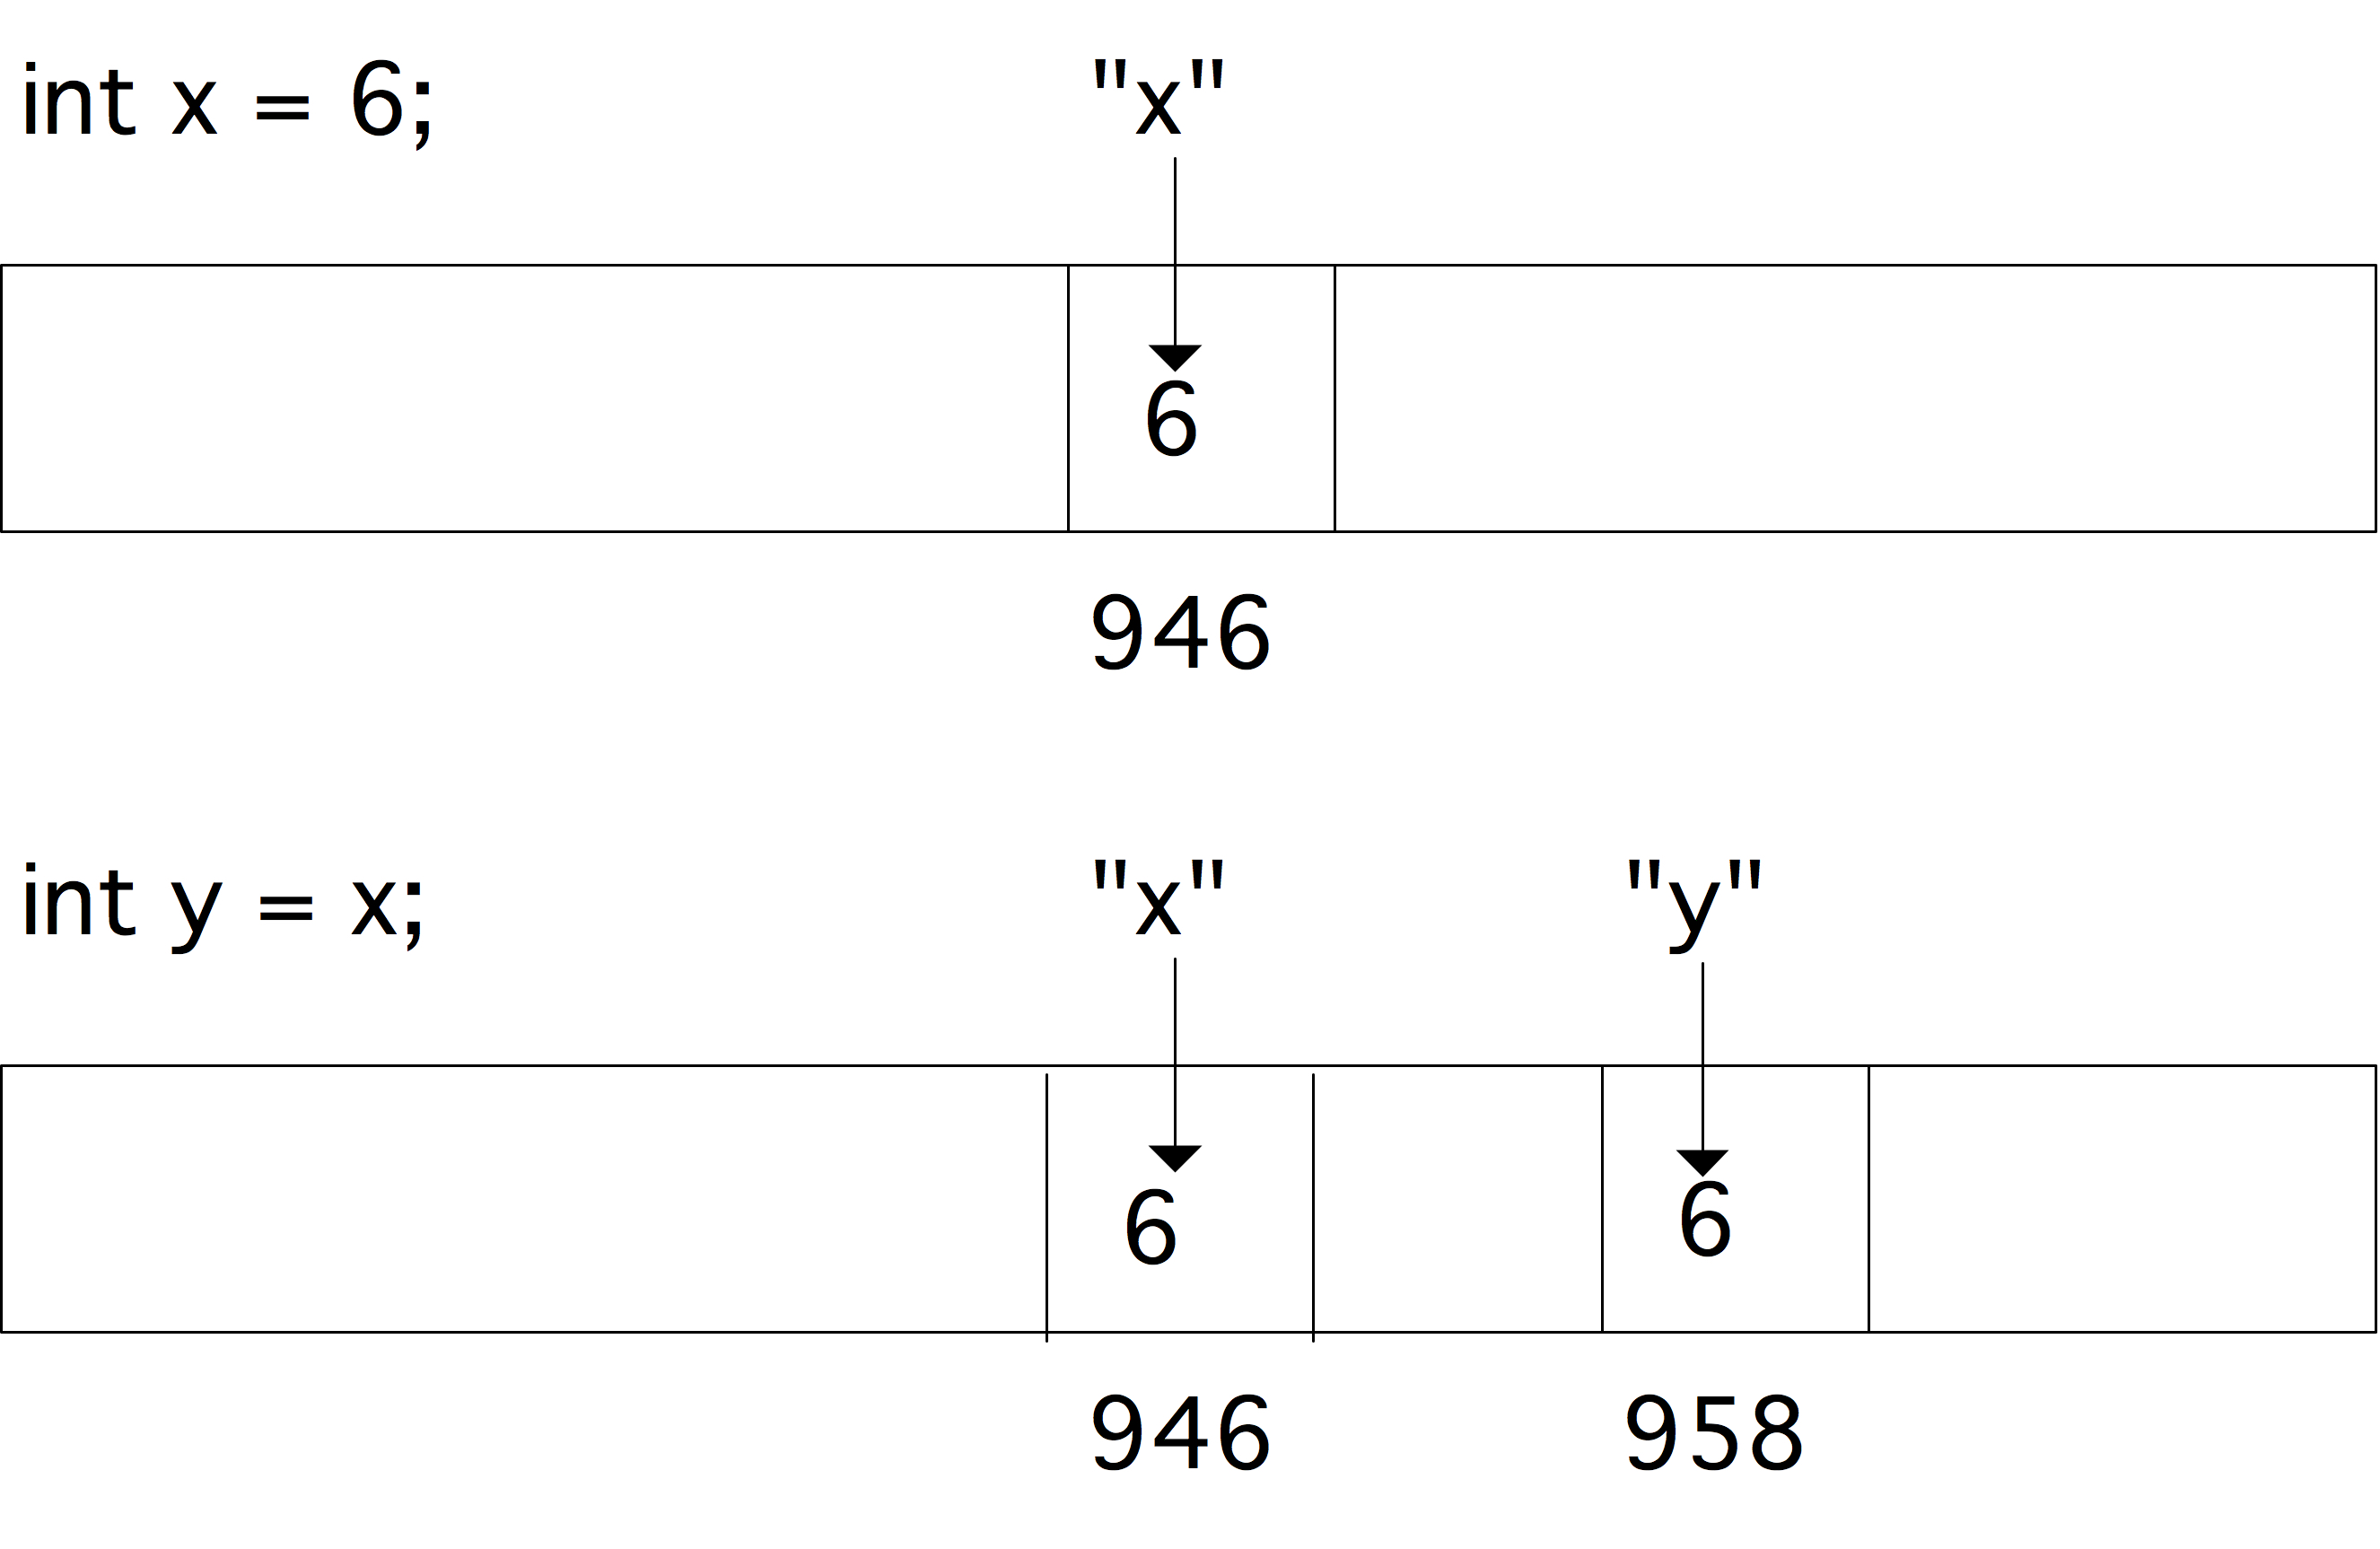
\includegraphics[scale=.1]{intstar1}
\end{block}

\begin{block}{illustration}
  \label{sl:deref-pic}
  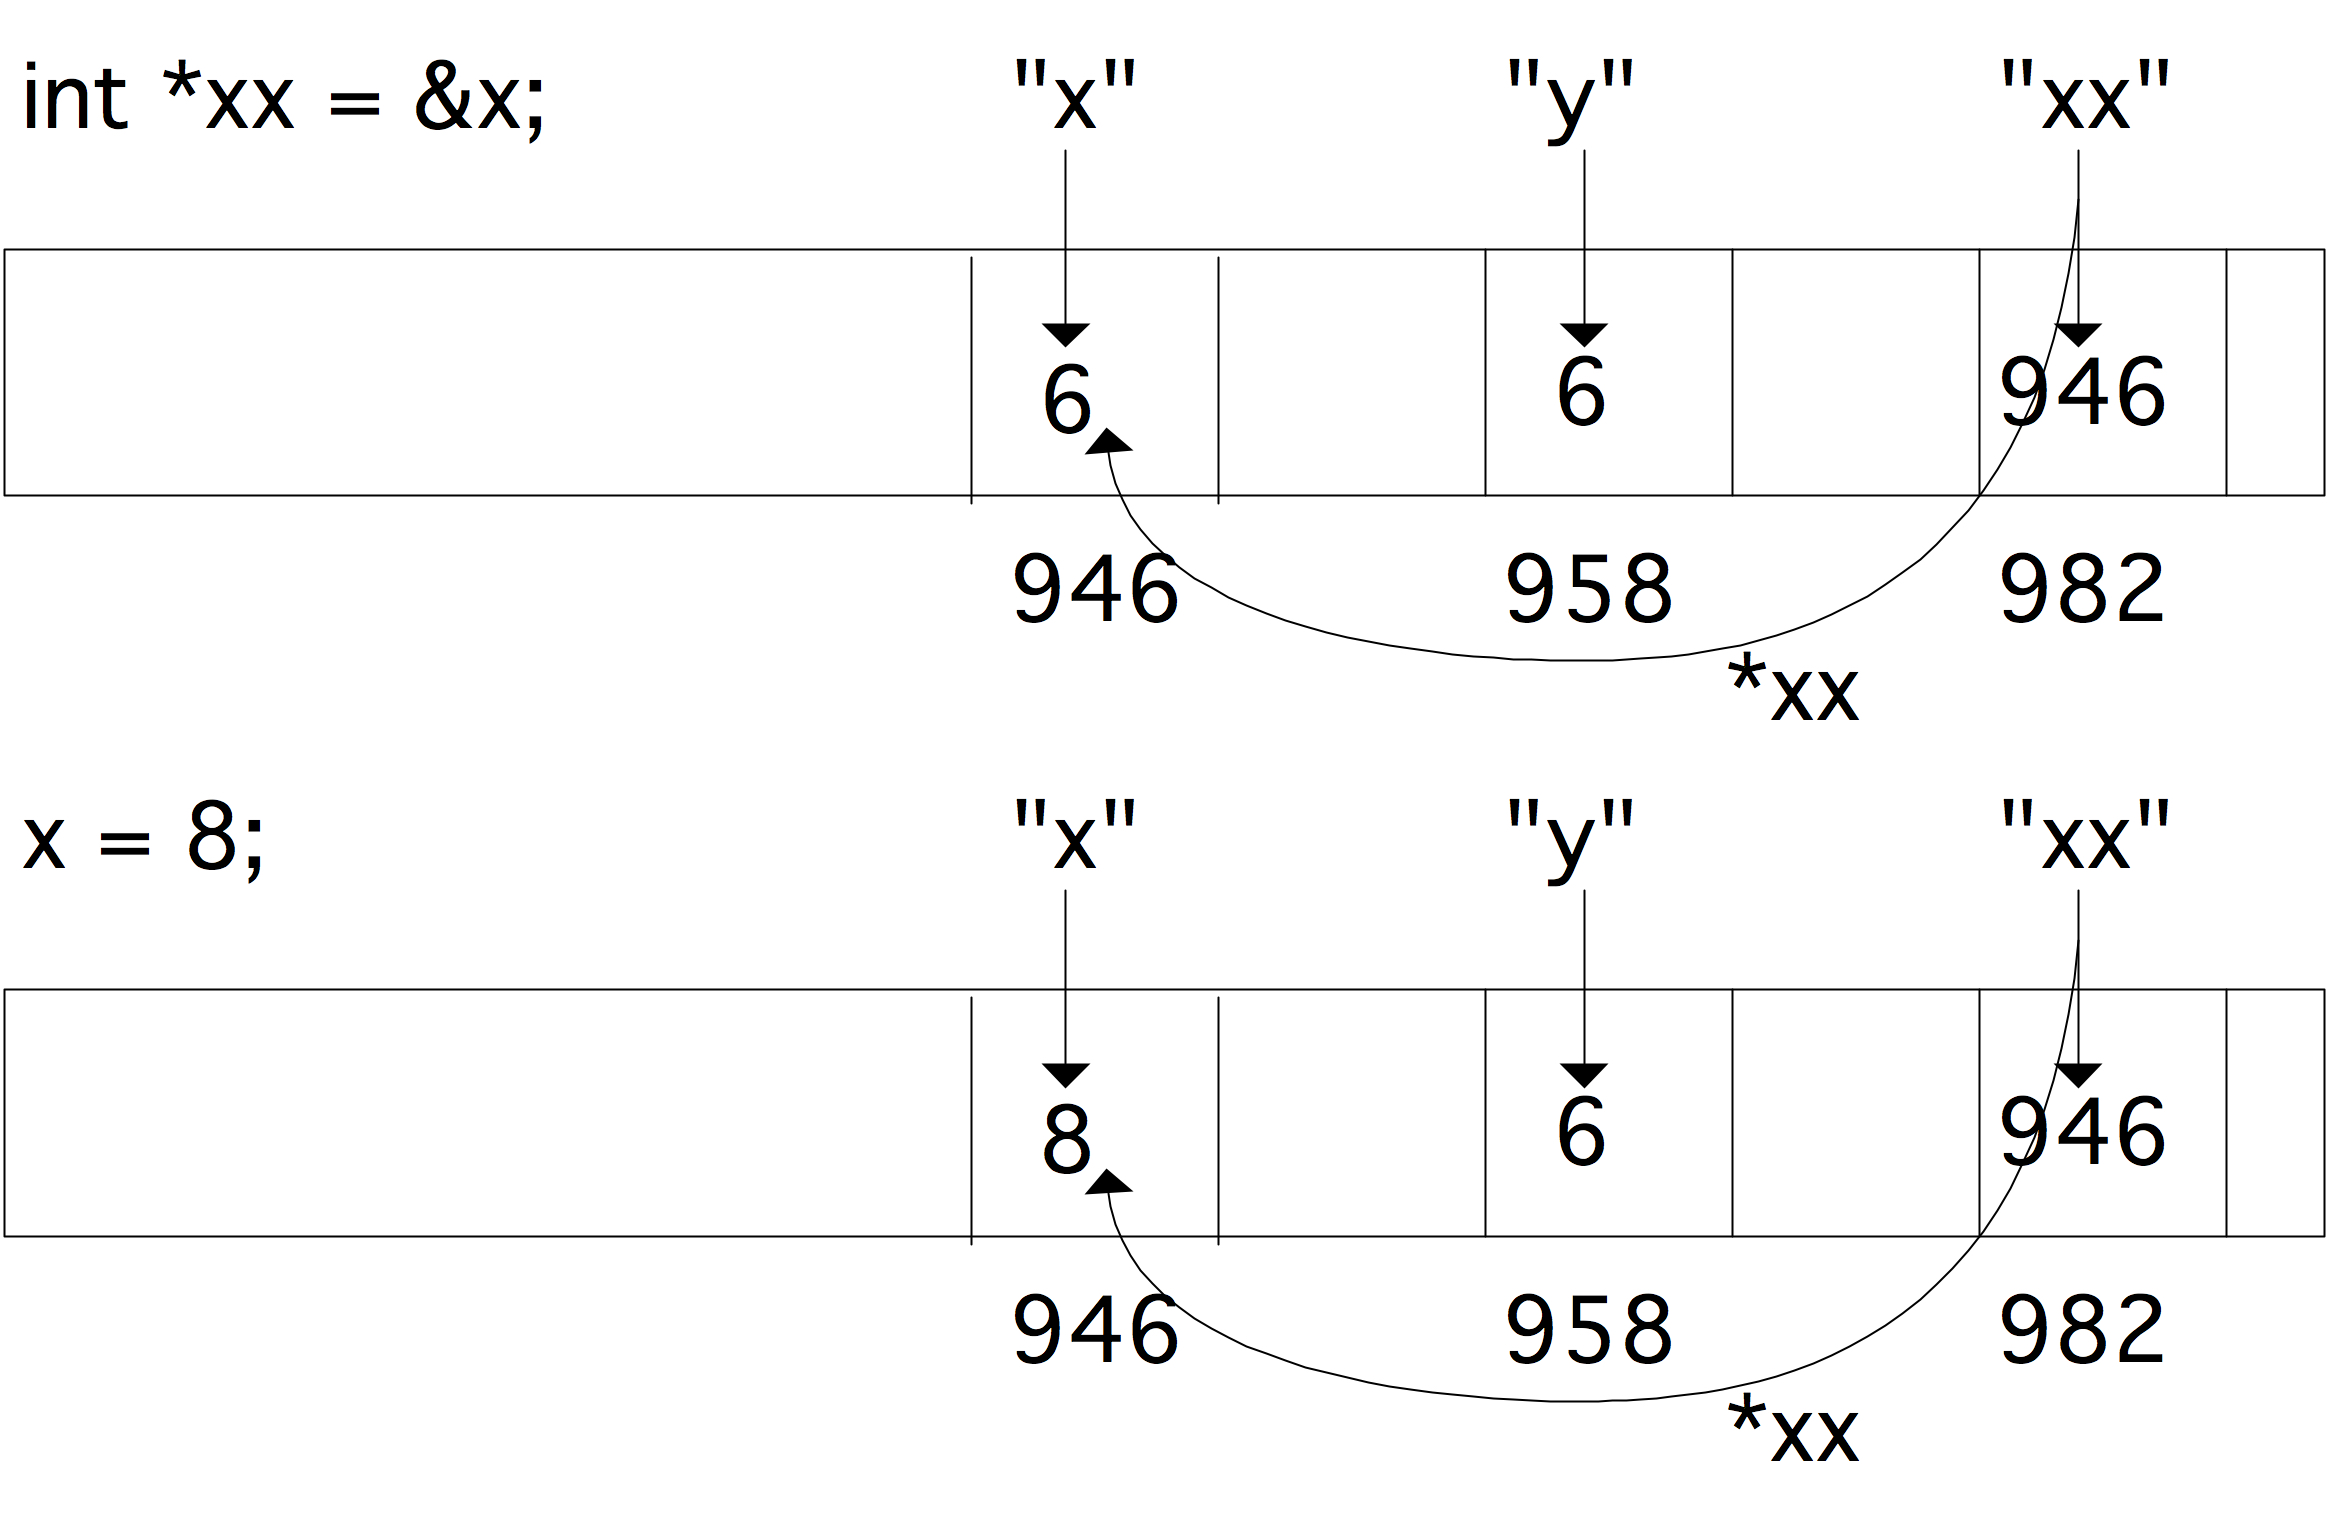
\includegraphics[scale=.1]{intstar2}
\end{block}

\begin{itemize}
\item \n{addr} is the address of~\n{i}.
\item You set \n{i} to~5; nothing changes about \n{addr}. This has the
  effect of writing \n{5} in the memory location of~\n{i}.
\item The first \n{cout} line dereferences \n{addr}, that is, looks up
  what is in that memory location.
\item Next you change \n{i} to~\n{6}, that is, you write \n{6} in its
  memory location.
\item The second \n{cout} looks in the same memory location as before,
  and now finds~\n{6}.
\end{itemize}

The syntax for declaring a pointer-to-sometype allows for a small
variation, which indicates the two way you can interpret such a declaration.

\begin{block}{Star stuff}
  \label{sl:starstuff}
  Equivalent:
  \begin{itemize}
  \item \n{int* addr}: \n{addr} is an int-star, or
  \item \n{int *addr}: \n{*addr} is an int.
  \end{itemize}
\end{block}

The notion \n{int* addr} is equivalent to \n{int *addr}, and
semantically they are also the same: you could say that \n{addr} is an
int-star, or you could say that \n{*addr} is an int.

\Level 1 {Arrays and pointers}
\label{sec:arraypointer}

In section~\ref{sec:staticarray} you saw the treatment of static
arrays in~C++. Examples such as:
%
\verbatimsnippet{arraypass}
%
show that, even though an parameters are normally passed by value, that is
through copying, array parameters can be altered. The reason for this
is that there is no actual array type, and what is passed is a pointer
to the first element of the array. So arrays are still passed by
value, just not the `value of the array', but the value of its
location.

So you could pass an array like this:
%
\verbatimsnippet{arraypassstar}

\begin{block}{Array and pointer equivalence}
  \label{sl:array-pointer}
  Array and memory locations are largely the same:
\begin{verbatim}
double array[5];
double *addr_of_second = &(array[1]);
array = (11,22,33,44,55);
cout << *addr_of_second;
\end{verbatim}
\end{block}

\begin{block}{Dynamic allocation}
  \label{sl:newstar}
  \n{new} gives a something-star:
\begin{verbatim}
double *x;
x = new double[27];
\end{verbatim}
(Actually, C uses \indextermttdef{malloc}, but that looks similar.)
\end{block}

\Level 1 {Pointer arithmetic}

\begin{block}{Pointer arithmetic}
  \indextermbus{pointer}{arithmetic} uses the size of the objects it
  points at:
\begin{verbatim}
double *addr_of_element = array;
cout << *addr_of_element;
addr_of_element = addr_of_element+1;
cout << *addr_of_element;
\end{verbatim}
Increment add size of the array element, 4~or~8 bytes, not~one!
\end{block}

\begin{exercise}
  Write a subroutine that sets the i-th element of an array, but using
  pointer arithmetic: the routine should not contain any square brackets.
\end{exercise}

\Level 1 {Multi-dimensional arrays}

\begin{block}{Multi-dimensional arrays}
  \label{sl:static-multi}
After
\begin{verbatim}
double x[10][20];
\end{verbatim}
a row \n{x[3]} is a \n{double*}, so is \n{x} a \n{double**}?

Was it created as:
\begin{verbatim}
double **x = new double*[10];
for (int i=0; i<10; i++)
  x[i] = new double[20];
\end{verbatim}
No: multi-d arrays are contiguous.
\end{block}

\Level 1 {Parameter passing}

\begin{block}{C++ pass by reference}
  \label{sl:cpp-pass-ref}
  C++ style functions that alter their arguments:
\begin{verbatim}
void inc(int &i) { i += 1; }
int main() {
  int i=1;
  inc(i);
  cout << i << endl;
  return 0;
}
\end{verbatim}
\end{block}

\begin{block}{C-style pass by reference}
  \label{sl:c-pass-ref}
  In C you can not pass-by-reference like this. Instead, you pass the
  address of the variable~\n{i} by value:
\begin{verbatim}
void inc(int *i) { *i += 1; }
int main() {
  int i=1;
  inc(&i);
  cout << i << endl;
  return 0;
}
\end{verbatim}
Now the function gets an argument that is a memory address: \n{i}~is
an int-star. It then increases \n{*i}, which is an int variable, by one.
\end{block}

\begin{exercise}
  \label{ex:c-star-swap}
  Write another version of the \n{swap} function:
\begin{verbatim}
void swapij( /* something with i and j */ {
  /* your code */
}
int main() {
  int i=1,j=2;
  swapij( /* something with i and j */ );
  cout << "check that i is 2: " << i << endl;
  cout << "check that j is 1: " << i << endl;
  return 0;
}
\end{verbatim}
Hint: write C++ code, then insert stars where needed.
\end{exercise}

\Level 1 {Allocation}

In section~\ref{sec:staticarray} you learned how to create arrays that
are local to a scope:

\begin{block}{Problem with static arrays}
  \label{sl:no-static-alloc}
\begin{verbatim}
if ( something ) {
  double ar[25];
} else {
  double ar[26];
}
ar[0] = // there is no array!
\end{verbatim}
\end{block}

The array \n{ar} is created depending on if the condition is true, but
after
the conditional it disappears again. The mechanism of using
\indextermtt{new} (section~\ref{sec:arraynew}) allows you to allocate
storage that transcends its scope:

\begin{block}{Declaration and allocation}
  \label{sl:c-array-new}
\begin{verbatim}
double *array;
if (something) {
  array = new double[25];
} else {
  array = new double[26];
}
\end{verbatim}
(Size in doubles, not in bytes as in C)
\end{block}

\begin{block}{Memory leak1}
  \label{sl:leak1}
\begin{verbatim}
void func() {
  double *array = new double[large_number];
  // code that uses array
}
int main() {
  func();
};
\end{verbatim}
\begin{itemize}
\item
  The function allocates memory
\item After the function ends, there is no way to get at that memory
\item $\Rightarrow$ \indextermbusdef{memory}{leak}.
\end{itemize}

\end{block}

\begin{block}{Memory leaks}
  \label{sl:leak2}
\begin{verbatim}
for (int i=0; i<large_num; i++) {
  double *array = new double[1000];
  // code that uses array
}
\end{verbatim}
  Every iteration reserves memory, which is never released:
  another \indextermbus{memory}{leak}.

  Your code will run out of memory!
\end{block}

\begin{block}{De-allocation}
  \label{sl:c-array-del}
  Memory allocated with \n{new} does not disappear when you leave a
  scope. Therefore you have to delete the memory explicitly:
\begin{verbatim}
delete(array);
\end{verbatim}
The C++ \n{vector} does not have this problem, because it obeys scope rules.
\end{block}

\begin{block}{Stop using C!}
  \label{sl:no-c-malloc}
  No need for \n{malloc} or \n{new}
  \begin{itemize}
  \item Use \n{std::string} for character arrays, and
  \item \n{std::vector} for everything else.
  \end{itemize}
  No performance hit if you don't dynamically alter the size.
\end{block}

\Level 2 {Malloc}

The keywords \n{new} and \n{delete} are in the spirit of C~style
programming, but don't exist in~C. Instead, you use
\indextermtt{malloc}, which creates a memory area with a size
expressed in bytes. Use the function \indextermtt{sizeof} to translate
from types to bytes:

\begin{block}{Allocation in C}
\begin{verbatim}
int n;
double *array;
array = malloc( n*sizeof(double) );
if (!array)
  // allocation failed!
\end{verbatim}
\end{block}

\Level 2 {Allocation in a function}

The mechanism of creating memory, and assigning it to a `star'
variable
can be used to allocate data in a function and
return it from the function.

\begin{block}{Allocation in a function}
\begin{verbatim}
void make_array( double **a, int n ) {
  *a = new double[n];
}
int main() {
  double *array;
  make_array(&array,17);
}
\end{verbatim}
\end{block}

Note that this requires a `double-star' or `star-star' argument:
\begin{itemize}
\item The variable \n{a} will contain an array, so it needs to be of
  type \n{double*};
\item but it needs to be passed by reference to the function, making
  the argument type~\n{double**};
\item inside the function you then assign the new storage to the
  \n{double*} variable, which is~\n{*a}.
\end{itemize}
Tricky, I~know.

\Level 1 {Memory leaks}
\label{sec:memleak}

Pointers can lead to a problem called \indextermdef{memory leaking}:
there is memory that you have reserved, but you have lost the ability
to access it.

In this example:
\begin{verbatim}
double *array = new double[100];
// ...
array = new double[105];
\end{verbatim}
memory is allocated twice. The memory that was allocated first is
never release, because in the intervening code another pointer to it
may have been set. However, if that doesn't happen, the memory is both
allocated, and unreachable. That's what memory leaks are about.

\Level 0 {Safer pointers in C++}
\label{sec:shared_ptr}

Section~\ref{sec:memleak} showed how how memory can become
unreachable. The \indexterm{C++11} standard has mechanisms that can
help solve this problem\footnote{A mechanism along these lines already
  existed in the `weak pointer', but it was all but unusable.}.

A `shared pointer' is a pointer that keeps count of how many times the
object is pointed to. If one of these pointers starts pointing
elsewhere, the shared pointer decreases this `reference count'. If the
reference count reaches zero, the object is deallocated or destroyed.

\begin{block}{Shared pointers}
  \label{sl:shared-ptr}
Shared pointers look like regular pointers:
\begin{verbatim}
#include <memory>

std::shared_ptr<myobject> obj_ptr
    = std::shared_ptr<myobject>( new myobject(x) );
obj_ptr->mymethod(1.1);
cout << obj_ptr->member << endl;

auto array = std::shared_ptr<double>( new double[100] );
// ILLEGAL: array[1] = 2.14;
array->at(2) = 3.15;
\end{verbatim}
\end{block}

As an illustration, let's take a class that reports its construction
and destruction:
%
\begin{block}{Reference counting illustrated}
  \label{sl:construct-destruct-trace}
  We need a class with constructor and destructor tracing:
  \verbatimsnippet{thingcall}
\end{block}

%
and
\begin{block}{Trace1: pointer overwrite}
  \label{sl:shared-ptr-overwrite}
  Let's create a pointer and overwrite it:
  %
  \snippetwithoutput{shareptr1}{pointer}{ptr1}
\end{block}
%
You see that overwriting the pointer does not cause a
\indexterm{memory leak}, as would happen with C-style pointers, but
causes destruction of the object it points to.

Next we overwrite a pointer, but after having copied it. Now the
destructor will not be called until all references to the object
--~both the original pointer and the copy~-- have been overwritten.
%
\begin{block}{Trace2: pointer copy}
  \label{sl:shared-ptr-copy}
  \snippetwithoutput{shareptr2}{pointer}{ptr2}
\end{block}

\Level 1 {Shared from this}

There is a problem with shared pointers in the case where a method has
to produce a pointer. For instance, to program linked lists you want a
method:
\begin{slide}{Linked list code}
  \label{sl:share-ptr-node}  
\begin{verbatim}
node *node::prepend_or_append(node *other) {
  if (other->value>this->value) {
    this->tail = other;
    return this;
  } else {
    other->tail = this;
    return other;
  }
};
\end{verbatim}
Can we do this with shared pointers?
\end{slide}

\begin{block}{A problem with shared pointers}
  \label{sl:share-ptr-node-sh}
\begin{verbatim}
shared_pointer<node> node:prepend_or_append
    ( shared_ptr<node> other ) {
  if (other->value>this->value) {
    this->tail = other;
\end{verbatim}
So far so good. However, \n{this} is a \n{node*}, not a
\n{shared_ptr<node}, so
\begin{verbatim}
    return this;
\end{verbatim}
returns the wrong type.
\end{block}

\begin{block}{Solution: shared from this}
  \label{sl:share-ptr-node-from}
  Solution: define your node class with (warning, major magic alert):
\begin{verbatim}
class node : public enable_shared_from_this<node> {
\end{verbatim}
This allows you to write:
\begin{verbatim}
    return this->shared_from_this();
\end{verbatim}
\end{block}
